% ========== RINGDUE ==========
\begin{frame}{%
  \begin{minipage}[c]{0.30\textwidth}
    Ringdue
  \end{minipage}%
  \hfill
  \begin{minipage}[c]{0.45\textwidth}
    \footnotesize
    \textbf{Jagttid:} 11.\ november -- 31.\ januar
  \end{minipage}%
  \hfill
  \begin{minipage}[c]{0.15\textwidth}
    \noindent\raggedleft
    
\includegraphics[width=0.5cm, height=0.5cm, keepaspectratio]{Billeder/Ikoner/star.png}%
    \hspace{0.2em}%
    
\includegraphics[width=0.5cm, height=0.5cm, keepaspectratio]{Billeder/Ikoner/star.png}%
    \hspace{0.2em}%
    
\includegraphics[width=0.5cm, height=0.5cm, keepaspectratio]{Billeder/Ikoner/star.png}
  \end{minipage}%
}
  \vspace{0.25em}
  \begin{columns}[T]
    \column{0.45\textwidth}
    \setlength{\parskip}{0.45em}
    \tiny
    \RaggedRight
    \textbf{\textit{Columba palumbus}} – mest almindelige due i Danmark, også kaldet skovdue \par
    \textbf{Udseende:}\\
    \quad – Gråblå fjerdragt \\
    \quad – Hvid halsplet \\
    \quad – Gult næb \par
    \textbf{Levesteder:} Alle landskabstyper, hyppigst nær byer. \par
    \textbf{Føde:} Plantefrø og landbrugsafgrøder. \par
    \textbf{Udbredelse:} Hele Danmark. \par
    \textbf{Træk/standfugl:} Begge \par
    \textbf{Forplantning:}\\
    \quad – \textbf{Yngleforhold:} Bygger enkel rede af kviste \\
    \quad – \textbf{Kønsmoden:} 1 år \\
    \quad – \textbf{Mono/polygam:} Monogam \\
    \quad – \textbf{Bestandsomsætning:} Hurtig \\
    \quad – \textbf{Kuld:} 2 æg, 2--4 gange om året
    \column{0.52\textwidth}
    \centering
    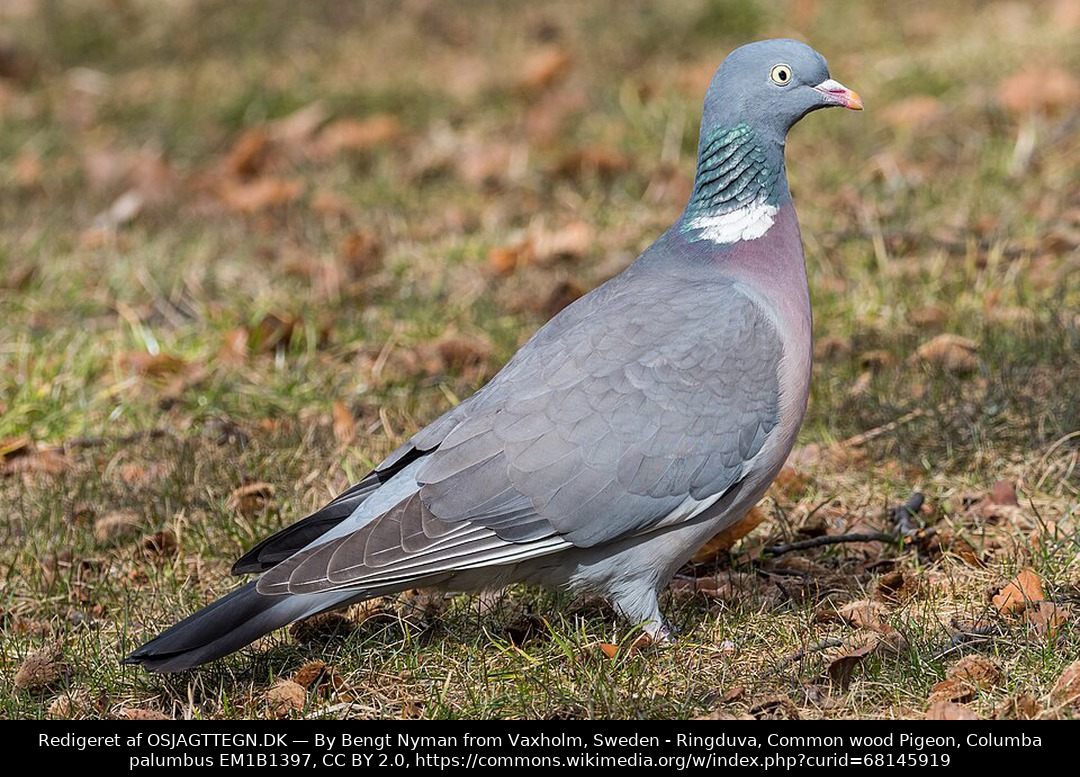
\includegraphics[width=\linewidth, height=7.2cm, keepaspectratio]{Billeder/Dyr/Fugle/Duer/ringdue-01.jpg}
  \end{columns}
\end{frame}